\chapter{Results}

\section{Torque estimation}
All four NN models were tested against various datasets. Using the angle data and 
physiological parameters of the user, actual torque was calculated. Then, model 
predicted torque was plotted against it.  

As illustrated in Figures \ref{fig:ovc0g}, \ref{fig:ovc0gstops} and \ref{fig:ovc10kg} 
the $closed\_model$ beats the $open\_model$ in terms of accuracy but neither 
achieve satisfactory results for higher loads. In fact, these models were trained 
on a dataset where a load of 900g was used and they work best on datasets with 
similar loads. The biggest advantage of the $closed\_model$ over the $open\_model$ 
is its better performance on the dataset containing stops illustrated in Figure 
\ref{fig:ovc0gstops}.  
\begin{figure}[htbp]
  \centering
  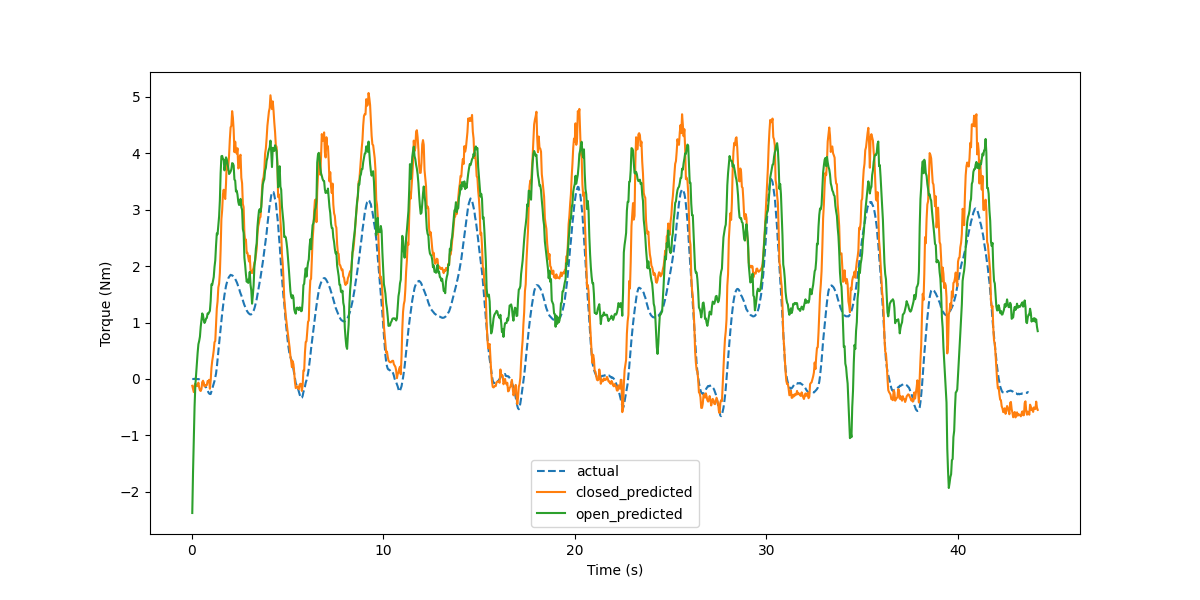
\includegraphics[width=\textwidth]{open_vs_closed_0g.png}
  \caption{No load}
  \label{fig:ovc0g}
\end{figure}
\begin{figure}[htbp]
  \centering
  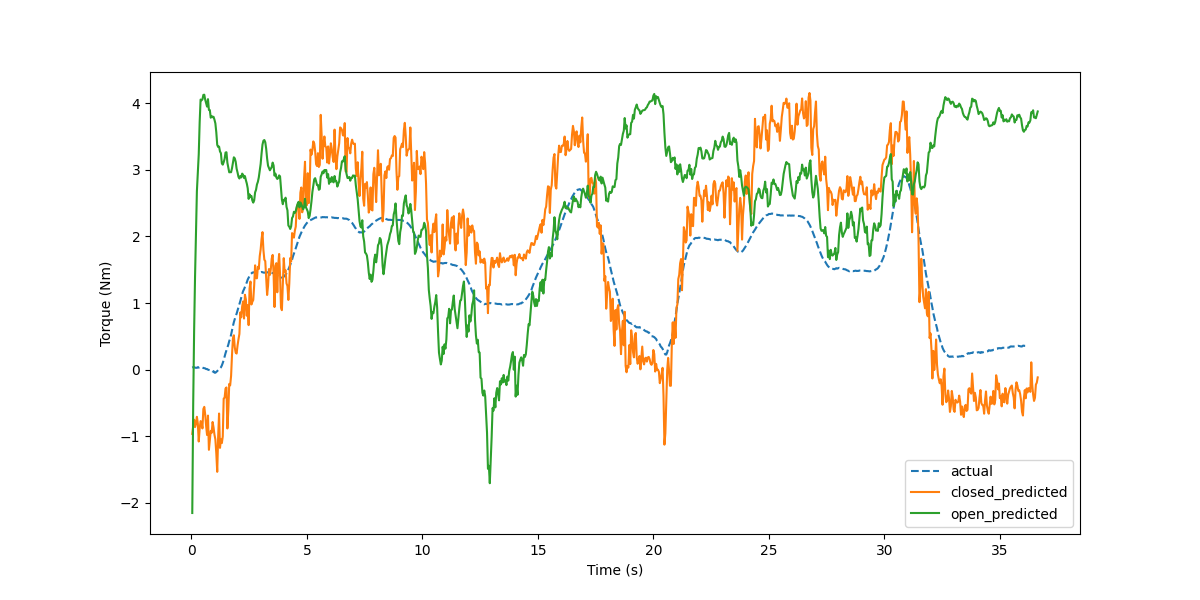
\includegraphics[width=\textwidth]{open_vs_closed_0g_stops.png}
  \caption{No load with stops}
  \label{fig:ovc0gstops}
\end{figure}
\begin{figure}[htbp]
  \centering
  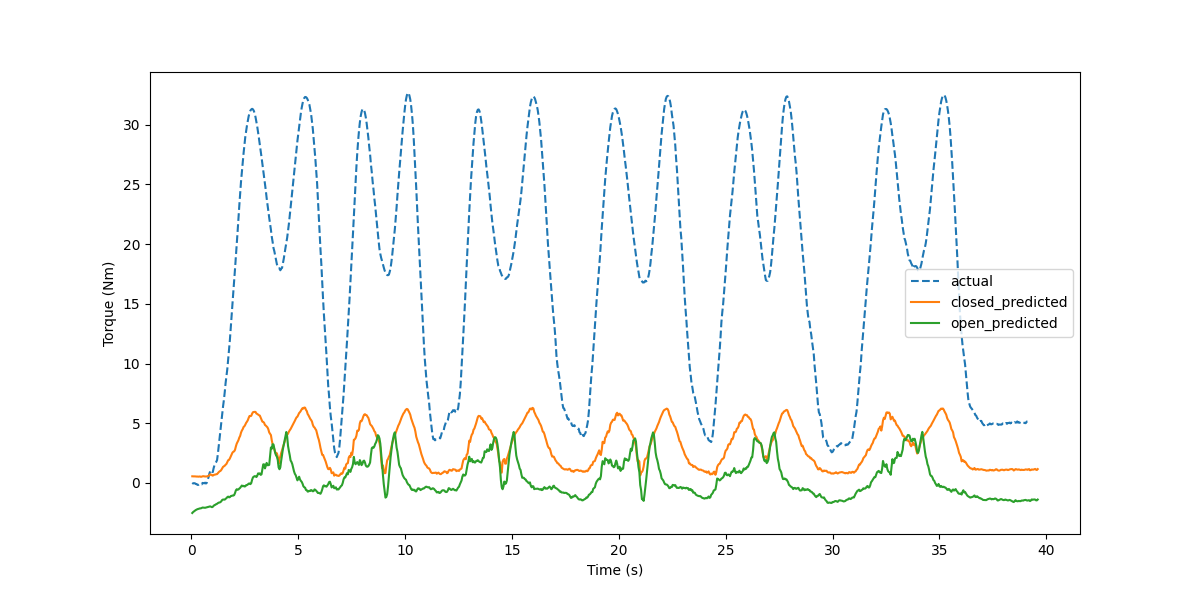
\includegraphics[width=\textwidth]{open_vs_closed_10kg.png}
  \caption{10kg load}
  \label{fig:ovc10kg}
\end{figure}

Models trained on all initial datasets showed no advantage over the first two 
models. As illustrated in Figures \ref{fig:movc0g}, \ref{fig:movcstops} and \ref{fig:movc10kg}, 
$multi\_open\_model$ and $multi\_closed\_model$ performed worse than their 
single-dataset counterparts.  

\begin{figure}[htbp]
  \centering
  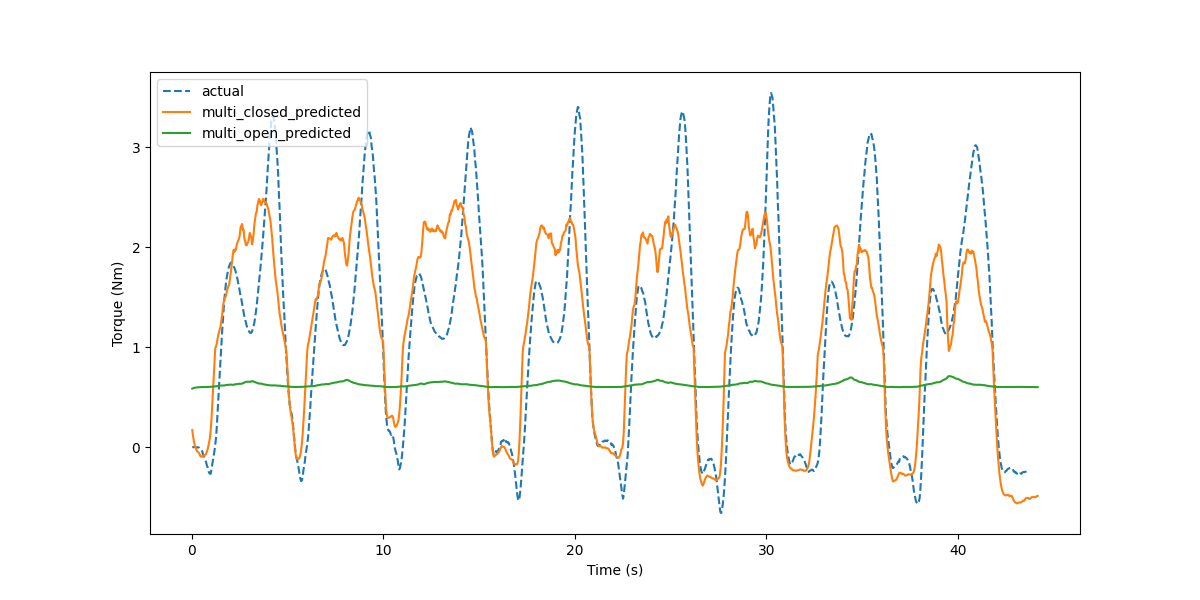
\includegraphics[width=\textwidth]{multi_open_vs_closed_0g.png}
  \caption{No load}
  \label{fig:movc0g}
\end{figure}
\begin{figure}[htbp]
  \centering
  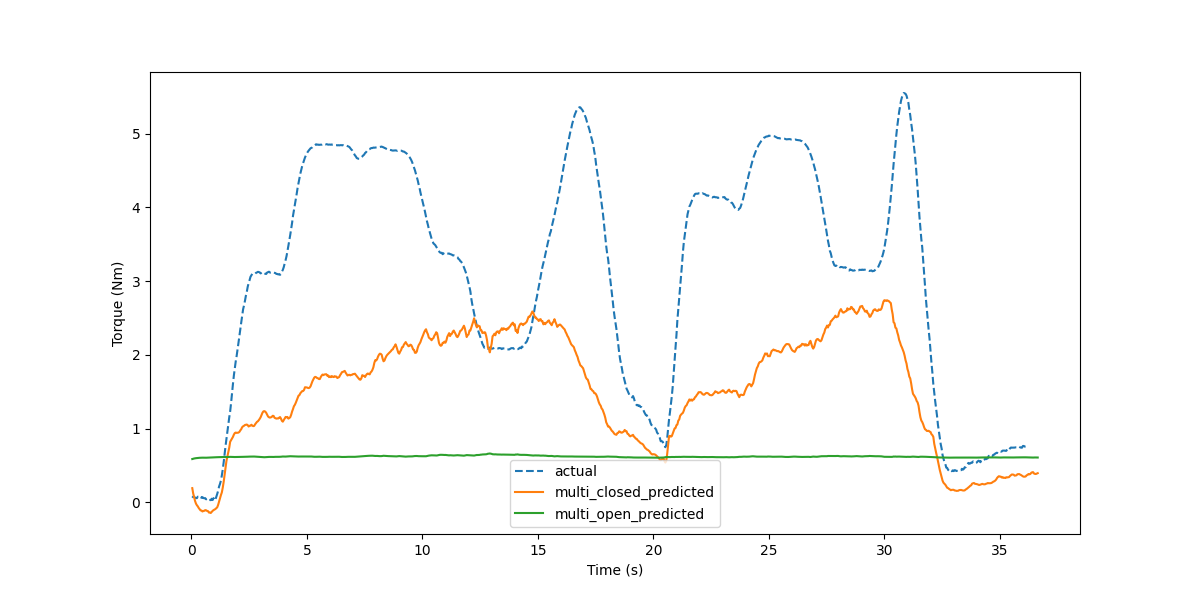
\includegraphics[width=\textwidth]{multi_open_vs_closed_stops.png}
  \caption{No load with stops}
  \label{fig:movcstops}
\end{figure}
\begin{figure}[htbp]
  \centering
  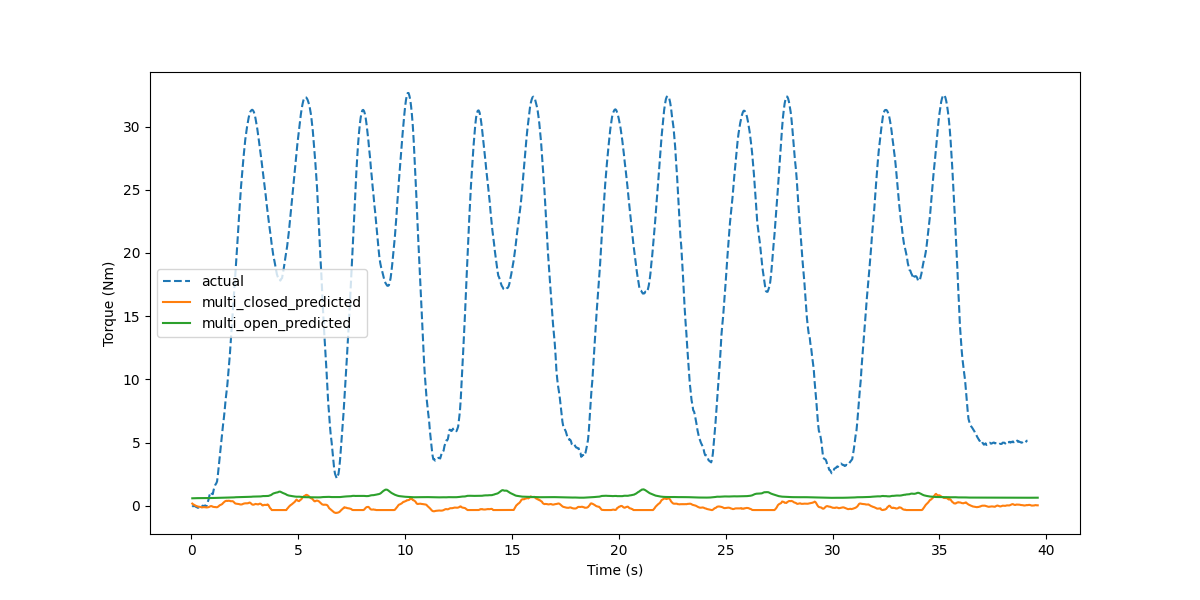
\includegraphics[width=\textwidth]{multi_open_vs_closed_10kg.png}
  \caption{10kg load}
  \label{fig:movc10kg}
\end{figure}
\FloatBarrier

\section{Experimental results}
The experimental setup is illustrated in Figure \ref{fig:setup}. The motor driver 
is first connected to the PC via USB, then the motor is securely tightened to the 
table surface and connected to the driver. The power supply is then also connected 
to the driver via a twisted pair power cable. Finally, the rope is tightened to 
prepare the system for testing.  

\begin{figure}[htbp]
  \centering
  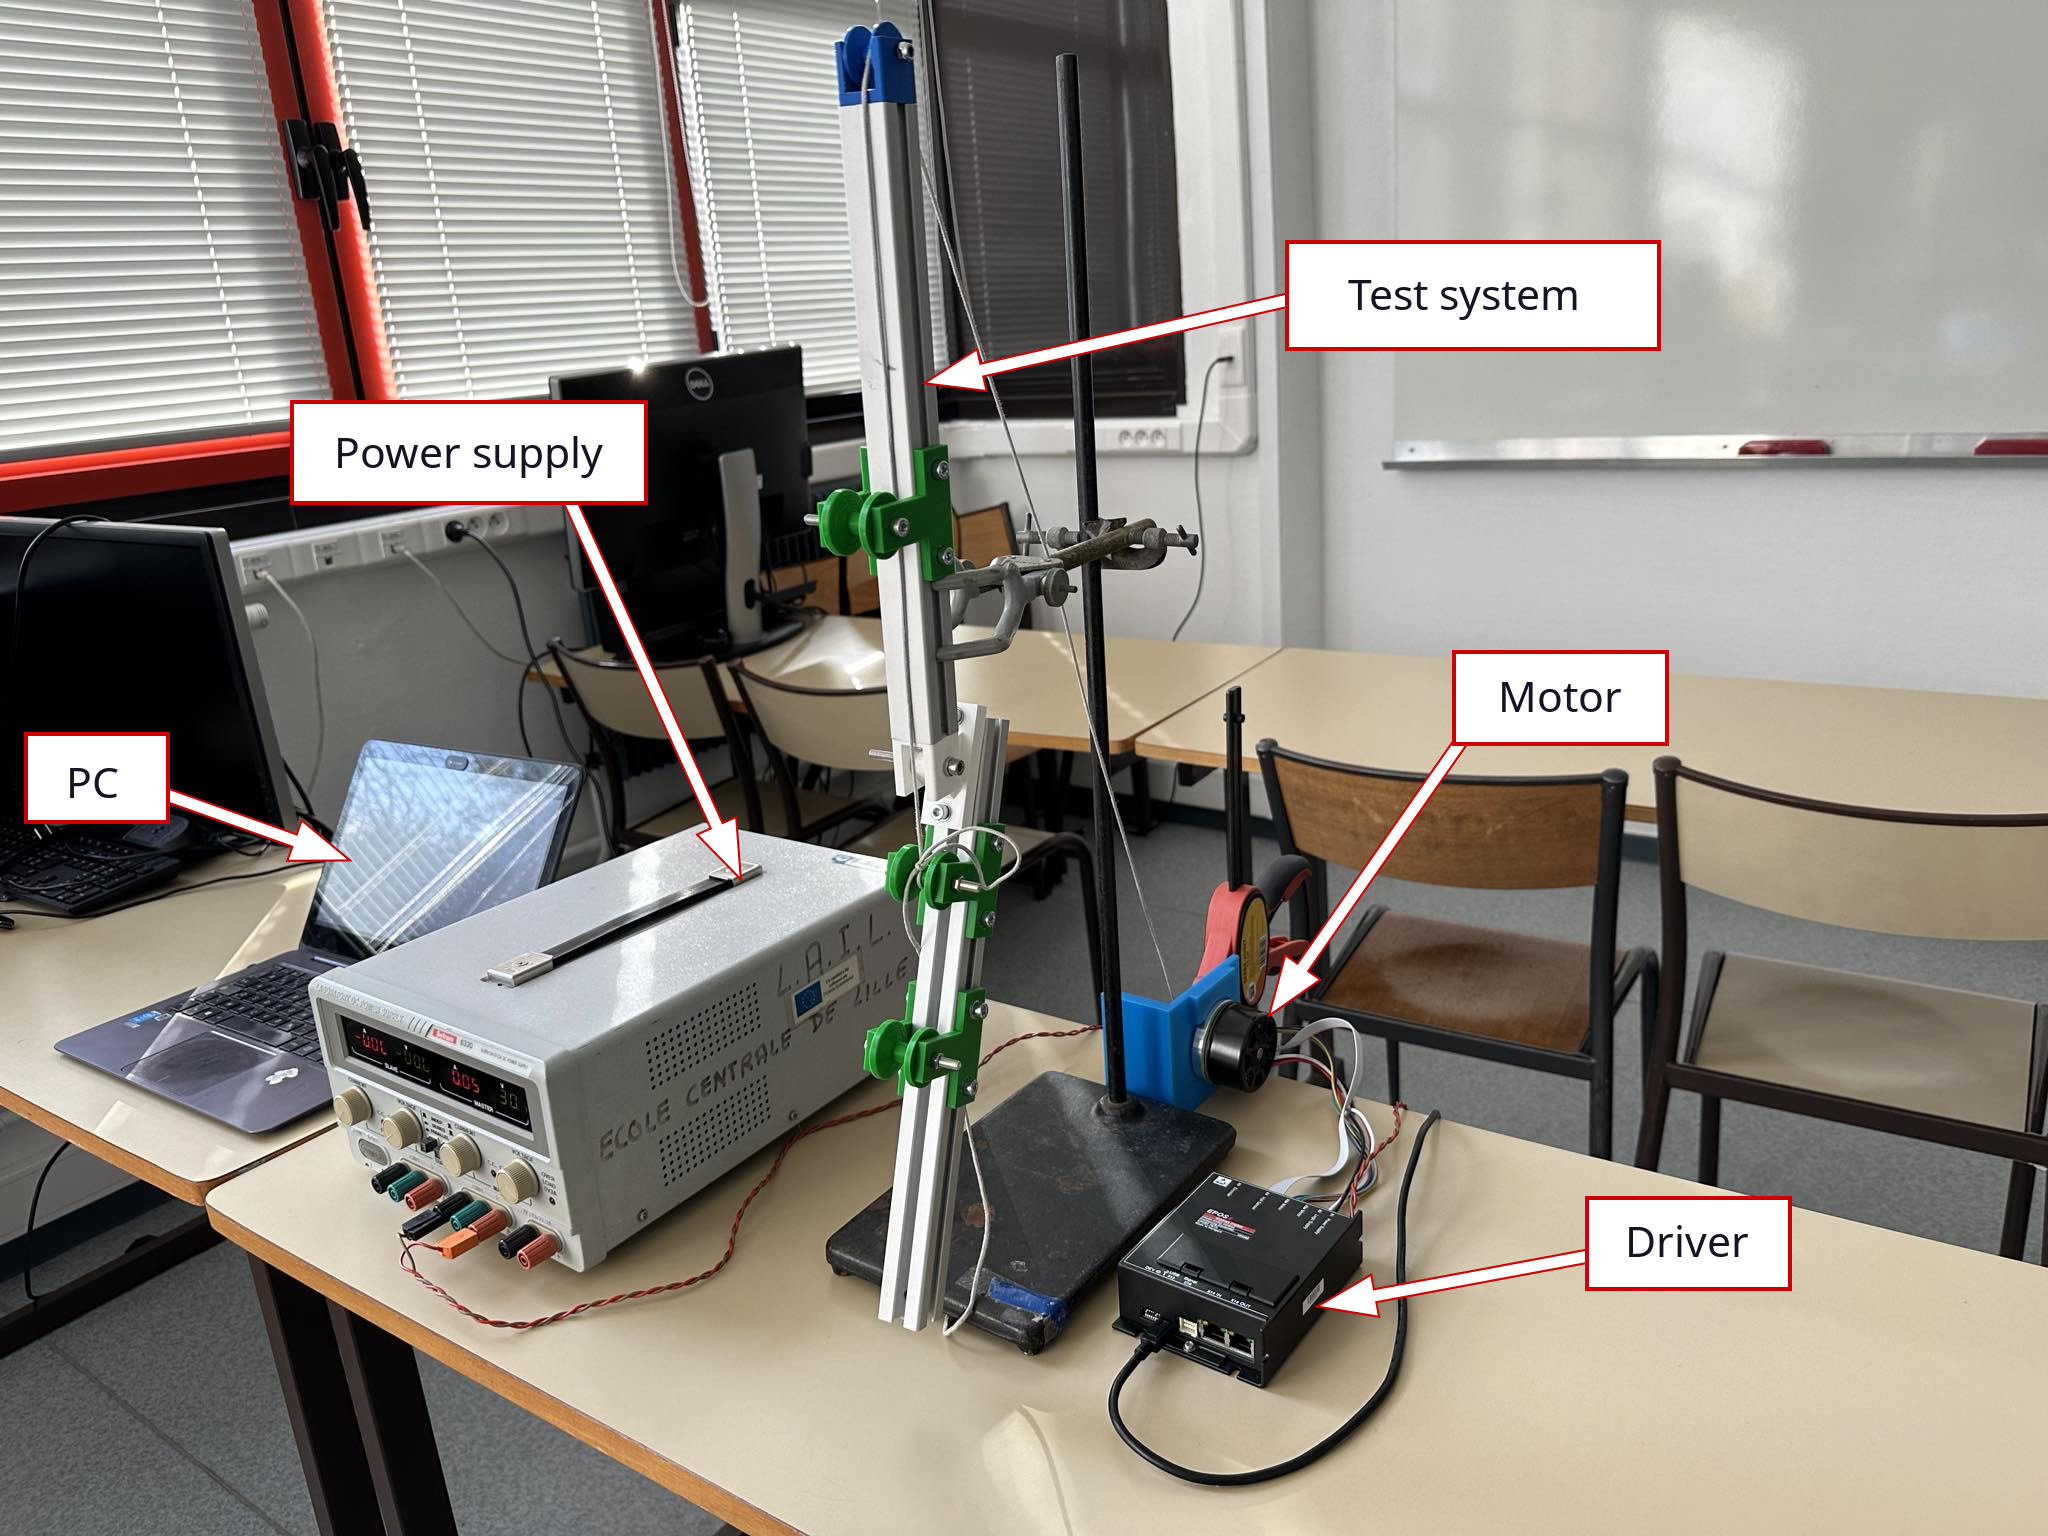
\includegraphics[width=0.6\textwidth]{setup.png}
  \caption{Experimental setup}
  \label{fig:setup}
\end{figure}
\FloatBarrier

\section{Experimental results}
